\chapter{Introduction}
\label{chapter:Introduction}
\thispagestyle{myheadings}

\section{Introduction} % needs this for some reason?

%% why dependent types?
Writing correct programs is difficult.
While many formal methods approaches make some errors rare or impossible, they often require programmers learn additional syntax and semantics.
Dependent type systems can offer a simpler approach.
In dependent type systems, proofs and properties use the same language and meaning already familiar to functional programmers.

While the type systems of mainstream programming languages allow tracking simple properties, like $\mathtt{7:int}$ or $\mathtt{not(x):bool}$.
Dependent types allow complicated properties to be assumed and verified, such as a provably correct sorting function

\[
sort\,:\,\left(input:List\,\mathbb{N}\right)\rightarrow\Sigma ls:List\,\mathbb{N}.IsSorted\,input\,ls
\]

by providing an appropriate definition of $sort$ at that type.
From the programmer's perspective, the function arrow and the implication arrow are the same.
The proof $IsSorted$ is no different than any other term of a datatype like $List$ or $\mathbb{N}$.

The power of dependent types has been recognized for decades.
Dependent types form the backbone of several poof systems, such as Coq\cite{Coq12}, Lean\cite{10.1007/978-3-030-79876-5_37}, and Agda\cite{norell2007towards}.
\todo{not clear these are the best citations, there seems to be little consensus online about how to cite software}
They have been proposed as a foundation for mathematics\cite{Martin-Lof-1972,HoTTbook}.
Dependent types are directly used in several programming languages such as ATS\cite{DependentMLAnapproachtopracticalprogrammingwithdependenttypes} and Idris\cite{brady2013idris}, while influencing many other programing languages such as Haskell and Scala.
\todo{cite the languages/ the dependent features both? neither?}

Unfortunately, dependent types have not yet become mainstream in the software industry.
Many of the usability issues with dependent types can trace their root to the conservative nature of dependently typed equality.
This thesis illustrates a new way to deal with equality constraints by delaying them until runtime.

A fragment of the system is proven correct according to a modified view of type soundness, and several of the proofs have been validated in Coq\footnote{
available at \url{https://github.com/marklemay/dtest-coq} most work is due to Qiancheng Fu}.
The system has been prototyped\footnote{available at \url{https://github.com/marklemay/dDynamic}}.

\todo[inline]{revise last paragraph? move?}

\subsection{Example}

Dependent type systems can prevent an index-out-of-bounds error when trying to read the first element of a list.
A version of the following type checks in virtually all dependent type systems:

\todo[inline]{expand this example? perhaps at the head of a constant vector first? ``and this reasoning can be abstracted under functions'' }

\begin{align*}
\mathtt{Bool} & :*,\\
\mathtt{Nat} & :*,\\
\mathtt{Vec} & :*\rightarrow\mathtt{Nat}\rightarrow*,\\
\mathtt{add} & :\mathtt{Nat}\rightarrow\mathtt{Nat}\rightarrow\mathtt{Nat},\\
\mathtt{rep} & :\left(A:*\right)\rightarrow A\rightarrow\left(x:\mathtt{Nat}\right)\rightarrow\mathtt{Vec\,}A\,x,\\
\mathtt{head} & :\left(A:*\right)\rightarrow\left(x:\mathtt{Nat}\right)\rightarrow\mathtt{Vec}\,A\,\left(\mathtt{add}\,1\,x\right)\rightarrow A
\end{align*}
\[
\vdash\lambda x.\mathtt{head}\,\mathtt{Bool}\,x\,\left(\mathtt{rep}\,\mathtt{Bool}\,\mathtt{true}\,\left(\mathtt{add}\,1\,x\right)\right)\,:\,\mathtt{Nat}\rightarrow\mathtt{Bool}
\]

\todo[inline]{make this a ``code'' example?}

Where $\rightarrow$ is a function and $*$ means that the function results in a type.
$\mathtt{Vec}$ is a list indexed by the type of element it contains and its length.
$\mathtt{Vec}$ is a type that depends on its length.
$\mathtt{rep}$ is a dependent function that produces a list containing a type with a given length by repeating its input that number of times.
$\mathtt{head}$ is a dependent function that expects a list of length $\mathtt{add}\,1\,x$, returning the first element of that non-empty list.

There is no risk that $\mathtt{head}$ inspects an empty list.
Luckily in the example the $\mathtt{\mathtt{rep}\,\mathtt{Bool}\,\mathtt{true}\,\left(\mathtt{add}\,1\,x\right)}$ function will return a list of length $\mathtt{add}\,1\,x$, exactly the type that is required.

%% This example only scratches the surface of what is possible with dependent types.

Unfortunately, programmers often find dependent type systems difficult to learn and use.
This resistance has limited the ability of dependent types to reach their full potential to help eliminate the bugs that pervade software systems.
One of the deepest underlying reasons for this frustration is the way dependent type systems handle equality.

For example, the following will not type check in any conventional dependent type system with user defined addition,

\[
\cancel{\vdash}\lambda x.\mathtt{head}\,\mathtt{Bool}\,x\,\left(\mathtt{rep}\,\mathtt{Bool}\,\mathtt{true}\,\left(\mathtt{add}\,x\,1\right)\right)\,:\,\mathtt{Nat}\rightarrow\mathtt{Bool}
\]

While ``obviously'' $1+x=x+1$, in the majority of dependently typed languages, $\mathtt{add}\,1\,x\equiv\mathtt{add}\,x\,1$ is not a ``definitional'' equality.
``Definitional equality'' is the name for the conservative approximation of equality used by dependent type systems for when two types are clearly the same.
This prevents the use of a term of type
$\mathtt{Vec}\,\mathtt{Bool}\,\left(\underline{\mathtt{add}\,1\,x}\right)$
where a term of type
$\mathtt{Vec}\,\mathtt{Bool}\,\left(\underline{\mathtt{add}\,x\,1}\right)$
is expected.
Usually when dependent type systems encounter situations like this, they will give an error message and prevent the programmer from doing more work until the ``mistake'' is resolved.

In programming, types are used to avoid bad behavior.
For instance, they are often used to avoid ``stuck'' terms.
If it is the case that $\mathtt{add}\,1\,x\,=\,\mathtt{add}\,x\,1$ the program will never get stuck.
However, if there is a mistake in the implementation of $\mathtt{add}$, then it is possible $\mathtt{add}\,1\,x\,\cancel{=}\,\mathtt{add}\,x\,1$ and the program might get stuck.
For instance, if the $\mathtt{add}$ function incorrectly computes $\mathtt{add}\,8\,1=0$ the above function will ``get stuck'' on the input $8$.

While the intent and properties of the $\mathtt{add}$ function are clear to programmers from its name and type, this information is unavailable to the type system.
If the programmer made a mistake in the definition of addition, such that for some $x$, $\mathtt{add}\,1\,x\,\cancel{=}\,\mathtt{add}\,x\,1$, the system will not provide hints on which $x$ witnesses this inequality.
Worse, the type system may even make it difficult to experiment with the $\mathtt{add}$ function, which makes repairing an actual bug difficult.

Why stop programmers when there is a definitional equality ``error''? \todo{Awk, in HM it makes sense to block}

There appears to be no reason! Alternatively, we can track unclear equalities and if the program ``gets stuck'', we are able to stop the program execution and provide a concrete witness for the inequality at runtime.
If the buggy add function above is encountered at runtime, we can give a runtime error stating $\mathtt{add}\,1\,8=9\,\neq\,0=\mathtt{add}\,8\,1$.
Which is exactly the kind of specific feedback programers want when fixing bugs.

\section{A Different Workflow}

This thesis advocates an alternative usage of types. In most types systems a programmer can't run programs until the type system is convinced of their correctness\footnote{
 often requiring a graduate degree and uncommon patience}.
Where this thesis argues ``the programmer is always right (until proven wrong)''.
This philosophy will likely go over better with programmers.

More concretely, whenever possible, static errors should be replaced with
\begin{itemize}
\item static warnings containing the same information,
\item and more concrete and clear runtime errors that correspond to one of the warnings
\end{itemize}
Figure \ref{fig:intro-standard-workflow} illustrates the standard workflow from the perspective of programmers in most typed languages.
Figure \ref{fig:intro-thesis-workflow} shows the workflow that is explored in this thesis.

\begin{figure}
% \begin{lstlisting}
% edit program
% |      ^
% |      | type errors
% v      |
% Type checks
% |
% | no type errors
% v
% run program
% \end{lstlisting}

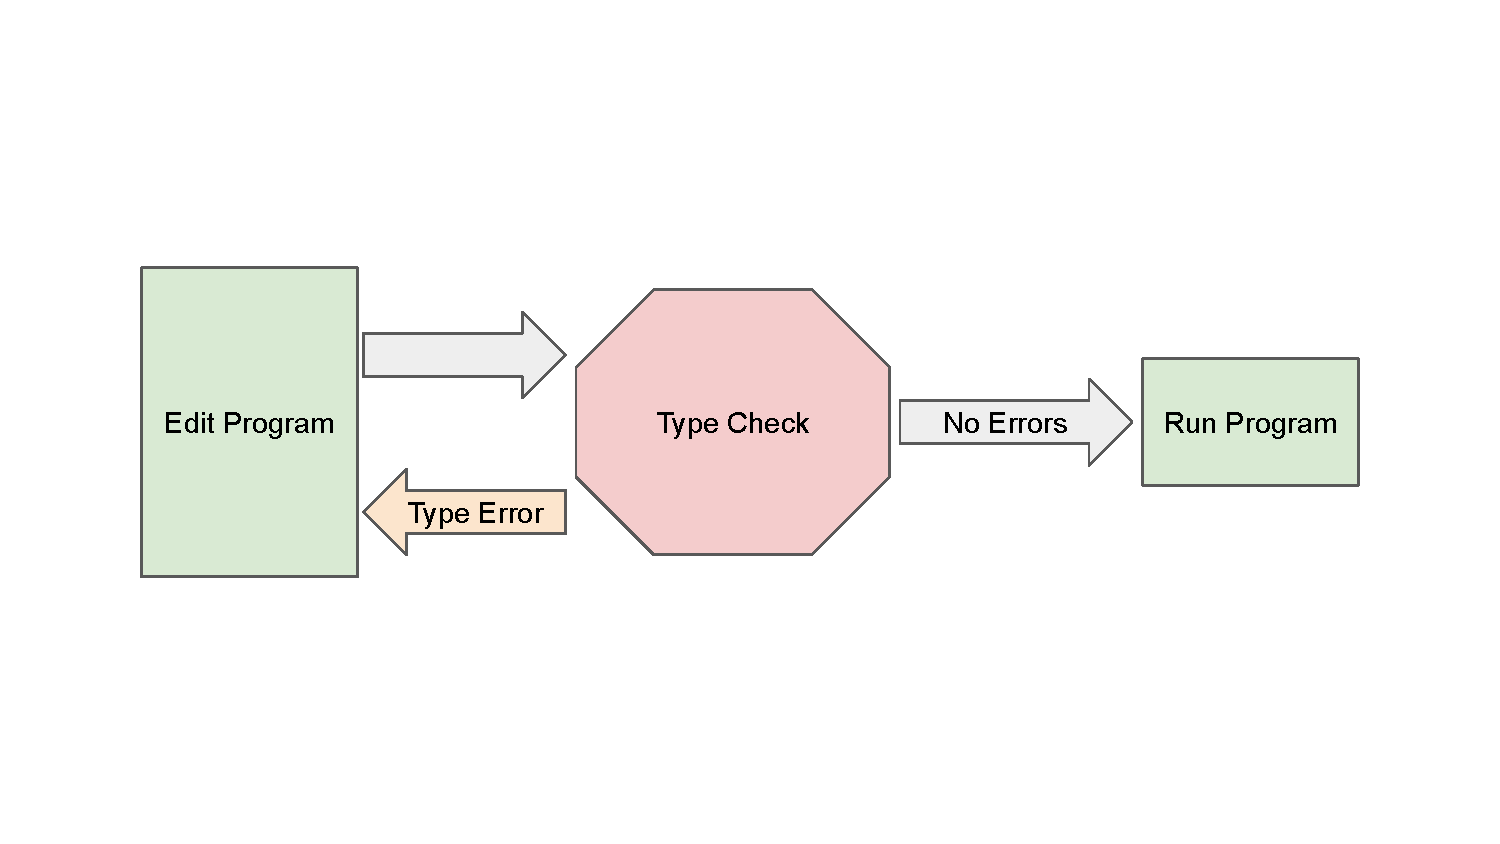
\includegraphics[width=5in]{1_intro/fig/standard-workflow.pdf}
% https://docs.google.com/presentation/d/1FSXDKsZlYFDNP8f6HprCrWV7gBRyW03PmIP0KkOprIA/edit#slide=id.g11561a4b8c2_0_0

\caption{Standard Typed Programming Workflow}
\label{fig:intro-standard-workflow}
\end{figure}

\begin{figure}
% \begin{lstlisting}
% edit program
% |     
% |     
% v
% Elaborates                     ^
% |              |               | runtime error
% | no warnings  | type warnings |
% v              v               |
%    run program   ---------------
% \end{lstlisting}
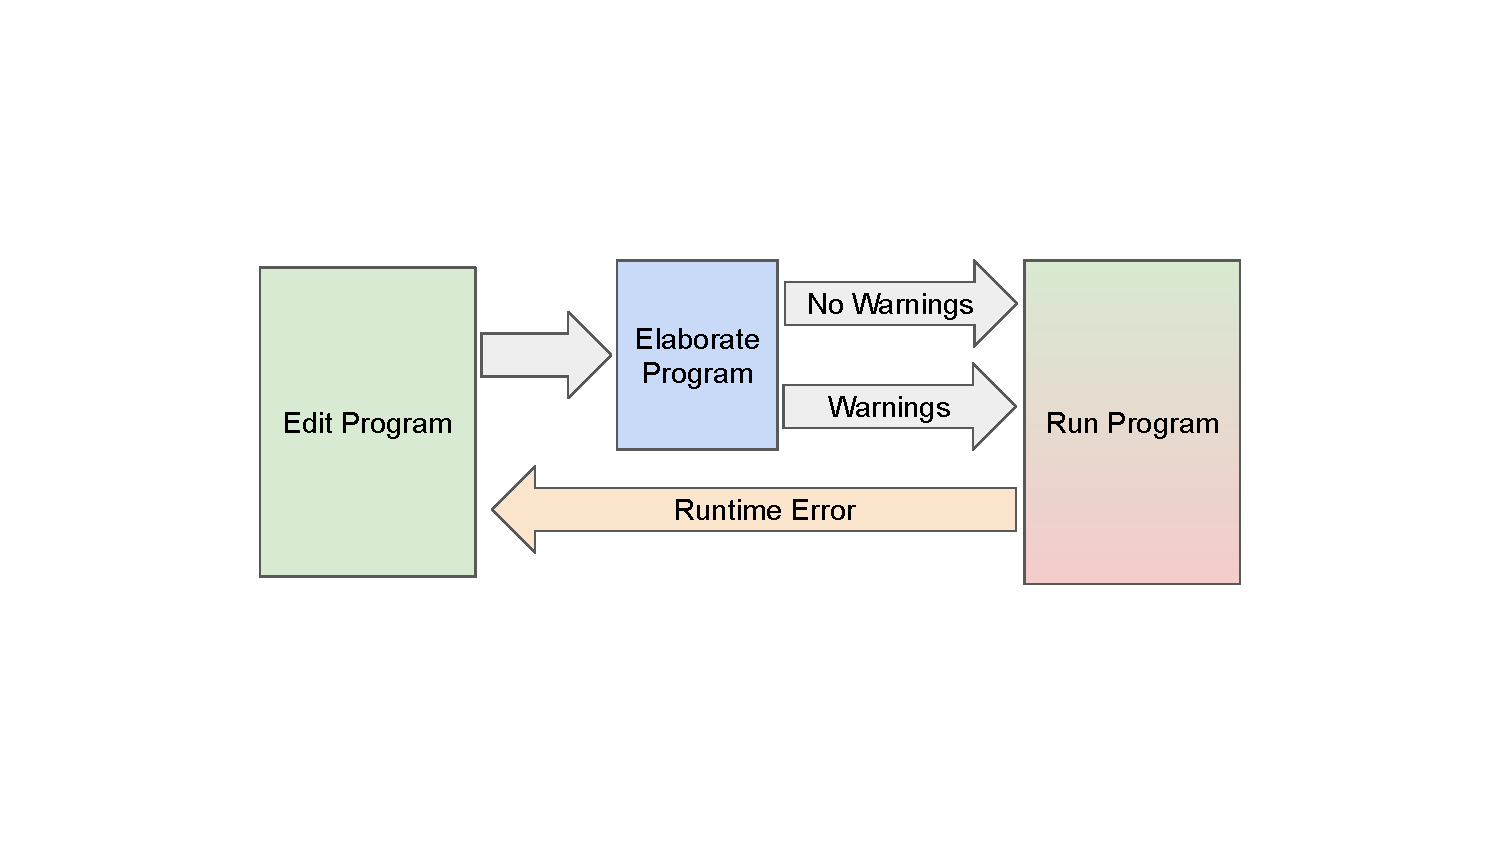
\includegraphics[width=5in]{1_intro/fig/new-workflow.pdf}
% https://docs.google.com/presentation/d/1FSXDKsZlYFDNP8f6HprCrWV7gBRyW03PmIP0KkOprIA/edit#slide=id.g11561a4b8c2_0_0

\caption{Workflow for this Thesis}
\label{fig:intro-thesis-workflow}
\end{figure}

These diagrams make it clear why there is so much pressure for type errors to be better in dependently typed programming\cite{eremondi2019framework}.
Type errors block programmers from running programs! However complaints about the type errors are probably better addressed by resolving the mismatch between the expectations of the programmer and the design of the underlying type theory.
Better worded error messages are unlikely to bridge this gap when the type system doubts $x+1=1+x$.

The standard workflow seems sufficient for type systems in many mainstream typed programming languages.
Though there is experimental evidence that even OCaml can be easier to learn and use with the proposed workflow \cite{10.1145/2951913.2951915}.
In the presence of dependent types the standard workflow is challenging for both beginners and experts, making a new approach much more critical.

\todo[inline]{
What is new here? talk about some of the prior dependent type attempts,
always a subset of syntax, or changes the syntax}

By switching to the proposed workflow, type errors become type warnings, and the programmer is free to run their program and experiment, while still presented with all the information they would have gotten from a type error (in the form of warnings).
If there are no warnings, the programmer could call their program a proof along the lines of the Curry-Howard correspondence\footnote{
  In the system presented here the programmer will need to manually verify termination
}\todo{cite?}.
If there is value in a type error it comes from the message itself and not the inconvenience it causes programmers.

The proposed workflow is necessary, since often the type system is too conservative and the programmer is correct in implicitly asserting an equality that is not provable within the system.
That the programmer may need to go outside the conservative bounds of definitional equality has been recognized since the earliest dependent type theories \cite{Martin-Lof-1972} and difficulties in dependently typed equality have motivated many research projects \cite{HoTTbook,sjoberg2015programming,cockx2021taming}.
However, these impressive efforts are still only usable by experts, since they frequently require the programmer prove their equalities explicitly\cite{HoTTbook,sjoberg2015programming}, or add custom rules into the type system \cite{cockx2021taming}.
Further, since program equivalence is undecidable in general, no system will be able to statically verify every ``obvious'' equality for arbitrary user defined data types and functions.
In practice, every dependently typed language has a way to assume equalities, even though these assumptions will result in computationally bad behavior (the program may ``get stuck'').

The proposed workflow presented in this thesis is justified by:
\begin{itemize}
\item The strict relation between warnings and runtime errors.
A runtime error will always correspond exactly to a reported warning, always validating the warning with a specific example.
\item A form of type soundness holds, programs will never ``get stuck'' unless a concrete witness of warning is found.
\item Programs that type check against a model type system will not have warnings, and therefore cannot have errors.
\item Other than warnings and errors the runtime behavior is similar to a conventional type theory.
% this is actually true, even in a normalizing theory, the runtime behavior is standard
\end{itemize}

\subsection{Example}

While the primary benefit of this system is the ability to experiment more freely with dependent types, while still getting the full feedback of a dependent type system, it is also possible to encode examples that would be unfeasible in existing systems.
This comes from accepting warnings that are justified with external mathematical or programmatic intuition, even while being theoretically thorny in dependent type theory.

For instance, here is part of an interpreter for interpreter for System F\todo{cite?}\footnote{
 System F is one of the foundational systems used to study programming languages.
 It is possible to fully encode evaluation and proofs into Agda, but it is difficult if computation, like substitution, happens in a type.
 In our system, it is possible to start with the ideal type indexed encoding and build an interpreter, without proving any properties of substitution.
} that encodes the type of the term at the type level.
The step function asserts type preservation of the interpreter in its function signature.

\begin{figure}
\begin{lstlisting}[basicstyle={\ttfamily\small}]
Ctx : * ;
Ctx = Var -> Ty;

data Ty : * {
| tv : tVar -> Ty
| arr : Ty -> Ty -> Ty
| forall : Ty -> Ty
};

data Term : Ctx -> Ty -> * {
| V : (ctx : (Var -> Ty)) -> (x : Var) ->
Term ctx (ctx x)
| lam : (ctx : Ctx) ->
(targ : Ty) -> (tbod : Ty) ->
Term (ext ctx targ) tbod ->
Term ctx (arr targ tbod)
| app : (ctx : Ctx) ->
(arg : Ty) -> (bod : Ty) ->
Term ctx (arr arg bod) ->
Term ctx arg ->
Term ctx bod
| tlam : (ctx : Ctx) ->
(bod : Ty) ->
Term ctx bod ->
Term ctx (forall bod)
| tapp : (ctx : Ctx) ->
(targ : Ty) -> (tbod : Ty) ->
Term ctx (forall tbod) ->
Term (tSubCtx targ ctx) (tSubt targ tbod)
};

step : (ctx : Ctx) -> (ty : Ty) -> Term ctx ty ->
Term ctx ty ;
step ctx ty trm =
case trm <_ => Term ctx ty > {
| (app _ targ tbod (lam _ _ _ bod) a) =>
 sub ctx targ a tbod bod
| x => x
};
\end{lstlisting}

\todo[inline]{clean up, write out sub?}\caption{System F}
\label{fig:ex-sysf}
\end{figure}

It will generate warnings like the following
\todo{``It will generate the following warnings'' need to clean up some bugs here}
\begin{itemize}
\item $\mathtt{tbod}$ in $\mathtt{Term\ (tSubCtx\ targ\ ctx)\ (tSubt\ targ\ \underline{tbod})}$
may have the wrong type
\end{itemize}
First note that the program has assumed several of the standard properties of substitution.
Formalizing substitution in a dependent type theory is a substantial
\todo{this might be really underselling it, we are talking months of effort}
task\cite{10.1145/3293880.3294101}\todo{cite some of the libs}.
Informally substitution and binding is usually considered obvious and uninteresting, and little explanation is usually given\footnote{A convention that will be followed in this thesis}.

Second, the type contexts have been encoded as functions.
This would be a reasonable encoding in a mainstream functional language since it hides the uninteresting lookup information.
This encoding would be inadvisable in other dependently typed languages since equality over functions is so fraught.
Here we can rest on our intuition that functions that act the same are the same.

Finally it is perfectly possible that there is a bug in the code invalidating one of the assumptions.
There are two options for the programmer:
\begin{itemize}
\item reformulate the above code so that there are no warnings, formally proving all the required properties in the language (this is possible but would take prohibitive effort)
\item exercise the $step$ function using standard software testing techniques.
If the interpreter does not preserve types, then a concrete counter example can be found.
\end{itemize}
The programmer is free to choose how much effort should go into removing warnings.
But even if the programmer wanted a fully formally correct interpreter, it would still be wise to test the functions first before attempting such a proof.

\todo[inline]{For instance, if the following error is introduced, }

\todo[inline]{Then it will be possible to get the runtime error }

\section{Design Decisions}

There are many flavors of dependent types that can be explored, this thesis attempts to always use the simplest and most programmer friendly formulations.
Specifically,
\begin{itemize}
\item The type system in this thesis is a \textbf{full spectrum} dependent type system.
The full-spectrum approach is the most uniform approach to dependent type theory, computation behaves the same at the term and type level.
This is contrasted with a leveled theory where terms embedded in types may have different or limited behavior\footnote{this is the approach taken in ATS, and refinement type systems}.
The full-spectrum approach is popular with theorem provers and has been advocated by many authors \cite{10.1145/289423.289451,norell2007towards,brady2013idris,sjoberg2012irrelevance}.
While the full spectrum approach offers tradeoffs (it is harder to deal with effects), it seems to be the most predictable from the programmer's perspective.
\item Data types and pattern matching are essential to practical programming, so they are included in the implementation.
While it is theoretically possible to simulate data types via church encodings, they are too awkward for programmers to work with, and would complicate the runtime errors this system hopes to deliver.
To provide a better programming experience data types are built into the system and pattern matching is supported.
\item The theories presented in this thesis will allow unrestricted general recursion and thus allow non-termination.
While there is some dispute about how essential general recursion is,
\todo{that mcbride paper? often cited as ``Church\textquoteright s Thesis and Functional Programming'' (2004), but that paper hardly says that}
there is no mainstream general purpose programming language that restricts termination.
Allowing nontermination weakens the system when considered as a logic (any proposition can be given a nonterminating inhabitant).
This removes any justification for a type universe hierarchy, so the system will support \tit{}.
Similarly non-strict data definitions are allowed.
\item Aside from the non-termination and runtime errors mentioned above, effects will not be allowed.
Even though effects seem essential to mainstream programing, they are a very complicated area of active research that will not be considered here.
The language studied is a ``pure'' (in the sense  Haskell) functional language.
As in Haskell, effects can be simulated with other language constructs.
\end{itemize}
It is possible to imagine a system where a wide range of properties are held optimistically and tested at runtime.
However the bulk of this thesis will only deal with equality, since that relation is uniquely fundamental to dependent type systems.
Since computation can appear at the type level, and types must be checked for equality, dependent type theories must define what computations they intend to equate for type checking.
It would be premature to deal with any other properties until definitional equality is dealt with.

\section{Issues}

Inserting runtime equality checks into a dependent types system is easier said than done.
\begin{itemize}
\item In the presence of Dependent types, equality checks may drift into types.
What does it mean when a term is a list of length $\mathtt{Bool}$?
\item Terms can ``get stuck'' in new ways. 
What happens when an equality check is used as a function by being applied with an argument?
What happens when a check blocks a pattern match?
\item Equality is not decidable at many types, even in the empty context.
For instance, functions of type $\mathtt{Nat}\rightarrow\mathtt{Nat}$ do not have decidable equality.
Therefore the types that embed them do not have decidable equality.
\end{itemize}
These problems are solved by extending dependent type theory with a cast checking operator.
This cast operator will ``get stuck'' if there is a discrepancy, and we can show that a program will always resolve to a value or get stuck in such a way that a counterexample can be reported.
\begin{itemize}
\item A system is needed to localize casts, these can be generated by extending a \textbf{\bidir{}} typing procedure to insert checks when it would statically check equality.
Without a reasonable way to localize checks, the work in this thesis would be infeasible.
\item When an argument is applied to a cast operator, new casts can be computed. % using similar logic to that of contracts and monitors\cite{10.1145/581478.581484}.
\item Once the casts are inserted, evaluations are possible.
Lazy evaluation means checking only has to happen up to the outermost type constructor, avoiding issues of undecidable equality.
\item Pattern matching can be extended to support equality evidence.
The branches of the pattern match can modify and use this evidence.
Unsatisfiable branches can redirect blame as needed.
\end{itemize}

\section{The Work in This Thesis}

% \begin{figure}
% \begin{lstlisting}[basicstyle={\ttfamily\tiny}]
% Surface language (ch. 2,4)
% {syntax {typed syntax {\bidir{}ly typed syntax}       }           }
%                       |                            |               |
% elaboration (ch. 3)   |without warnings            | with warnings |
%                       |                            |               |
%                       vvvvvvvvvvvvvvvvvvvvvvvvvvvvvvvvvvvvvvvvvvvvvv
%    {                   cast system (ch. 3)                             }

% \end{lstlisting}

% \todo[inline]{better graphics, ch 5}

% \caption{Systems in This Thesis}
% \label{fig:intro-thesis-workflow-1}
% \end{figure}

While apparently a simple idea, the technical details required to manage checks that delay until runtime in a dependently typed language is fairly involved.
To make the presentation easier, features will be added to the language in stages.

\todo[inline]{This should probably be expanded}
\begin{itemize}
\item Chapter 2 describes a dependently typed language (without data) intended to model standard dependent type theories, called the \textbf{Surface Language}.
\textbf{Type soundness} is proven and a \bidir{} type checking procedure system is presented.
Though the system is not original, the proof presented is the simplest complete progress and preservation style proof I am aware of for a dependent type system.   
\item Chapter 3 describes a dependently typed language (without data) with embedded equality checks, called the \textbf{cast language}.
The cast language has its own version of type soundness, called \textbf{cast soundness}.
Cast soundness is proven for the language, using a similar strategy to the type soundness proof of Chapter 2.
An Elaboration procedure takes most (untyped) terms of the surface syntax into terms in the cast language.
Several desirable properties for elaboration are presented. % and conjectured.
\item Chapter 4 reviews how dependent data and pattern matching can be added to the surface language and explores some of the issues of data in a dependent type system.
\item Chapter 5 shows how to extend the cast language with dependent data and pattern matching.
Surprisingly the inclusion of dependent data requires a much more complicated system then Chapter 3, since finer observations are observable.
\item Chapter 6 discusses other ideas related to usability and future work, such as automated testing and runtime proof search.
These systems are made feasible given the more flexible approach to equality addressed in the rest of the thesis.
\end{itemize}
Versions of the proof of type soundness in Chapter 2, and the cast soundness in Chapter 3 have been formally proven in Coq.
% Properties in chapter 4 and 5 are only conjectured correct.

Those interested in exploring the type soundness and type checking of a ``standard'' dependent type theory can read Chapters 2 and 4 which can serve as a self contained tutorial.
